% !TEX TS-program = xelatex
% !TEX encoding = UTF-8 Unicode
% !Mode:: "TeX:UTF-8"

\documentclass{resume}
\usepackage{zh_CN-Adobefonts_external} % Simplified Chinese Support using external fonts (./fonts/zh_CN-Adobe/)
%\usepackage{zh_CN-Adobefonts_internal} % Simplified Chinese Support using system fonts
%\usepackage{bm}
%\ usepackage { graphicx } 
%\ graphicspath {  { my / }  }
\usepackage[export]{adjustbox}
\usepackage{linespacing_fix} % disable extra space before next section
\usepackage{cite}
\usepackage{wrapfig}

\begin{document}
\pagenumbering{gobble} % suppress displaying page number

%\name{宋方腾}
%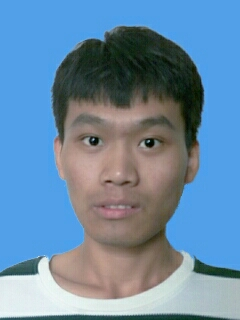
\includegraphics[width=0.9\linewidth, width=3cm,height=4cm, right]{photo}
%\basicInfo{
 %%\qquad\ 
  %\phone{157-356-58378} %\textperiodcentered\
  %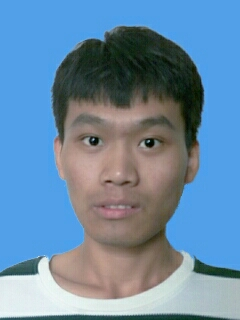
\includegraphics[width=0.9\linewidth, width=3cm,height=4cm, right]{photo}
  %\linkedin[billryan8]{https://www.linkedin.com/in/billryan8}
  %}%\\ \\  \\ \\
  %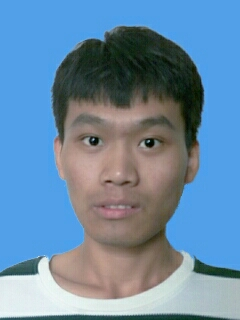
\includegraphics[width=3cm, height=4cm]{photo}
\begin{minipage}{0.65\textwidth}
\begingroup
\let\center\flushleft
\let\endcenter\endflushleft
\name{宋方腾}
\bigbreak
%\phone{157-356-58378}\\
%\email{2656713969s@gmail.com}
%\homepage{https://fmzhao.github.io}
\basicInfo{
  \email{songfangt@gmail.com} \qquad  \qquad \quad\ \phone{157-356-58378} %\textperiodcentered\ 
  %\linkedin[billryan8]{https://www.linkedin.com/in/billryan8}
  }
\endgroup
\end{minipage}
\raggedleft{
\begin{minipage}{0.3\textwidth}
\flushright{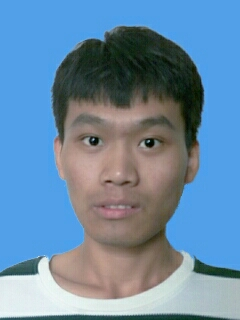
\includegraphics[width=65pt]{photo}}
\end{minipage}
}
%%%%%%%%%%%%%%%%%%%%%%%%%%%%%%%%
\section{\faHome\ 基本信息}
%\datedsubsection{\textbf{性别:}男}{出生年月:1996年4月}{籍贯:山东省枣庄市}
%\textit{\large{姓名:宋方腾}}\qquad  \qquad \qquad  \qquad \qquad 
\raggedright{\textit{\large{性别:男}}}\\ %\qquad  \qquad \qquad  \qquad \quad 
\textit{\large{出生年月:1996年04月}} \\%\qquad  \qquad \qquad  \qquad \qquad 
\textit{\large{籍贯:山东$ \cdot $枣庄}}\\%\qquad  \qquad \qquad  \qquad \qquad  
\textit{\large{地址:太原市尖草坪区中北大学文瀛一354室$|$ 030051}}
%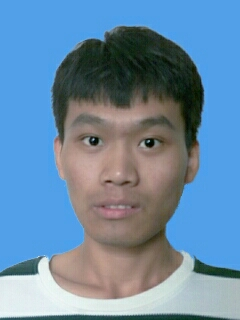
\includegraphics[width=0.9\linewidth, width=3cm,height=4cm, right]{photo}




\section{\faGraduationCap\  教育背景$\&$成绩}
\datedsubsection{\textbf{中北大学}, 太原}{2015年 -- 至今}
%\textit{在读硕士研究生}\ 信息与通信工程, 预计 2015 年 3 月毕业
%\datedsubsection{\textbf{西安电子科技大学}, 西安, 陕西}{2009 -- 2013}
\textit{\large{专业:}}\ 机械设计制造及其自动化(2015级) \\
\textit{\large{专业排名:2/146}} \ (本科前五学期) \\
%\textit{\large{前三年加权成绩:}}\\
\textit{\large{绩点:4.12}}

\section{\faCogs\ 个人技能}
%\datedsubsection{\textbf{黑科技公司} 上海}{2015年3月 -- 2015年5月}
%\role{实习}{经理: 高富帅}
%xxx后端开发
\begin{itemize}
  \item \textbf{英语水平:}\textbf{一次性}通过英语四级(572分),六级(488分)
  \item \textbf{计算机水平:}计算机二级
  \item \textbf{其它:}(1)全国爵士舞四级;(2)Pro/E$\&$CAD职业证书;(3)熟悉MATLAB、UG以及LaTeX,擅长Word,Excel。
\end{itemize}

%\datedsubsection{\textbf{分布式科学上网姿势}}{2014年6月 -- 至今}
%\role{Golang, Linux}{个人项目,和富帅糕合作开发}
%\begin{onehalfspacing}
%分布式负载均衡科学上网姿势, https://github.com/cyfdecyf/cow
%\item 修复了连接未正常关闭导致文件描述符耗尽的 bug
 %\item 使用Chord 哈希 URL, 实现稳定可靠地分流
  %\item xxx (尽量使用量化的客观结果)
%\end{itemize}
%\end{onehalfspacing}

%\datedsubsection{\textbf{\LaTeX\ 简历模板}}{2015 年5月 -- 至今}
%\role{\LaTeX, Python}{个人项目}
%\begin{onehalfspacing}
%优雅的 \LaTeX\ 简历模板, https://github.com/billryan/resume
%\begin{itemize}
  %\item 容易定制和扩展
  %\item 完善的 Unicode 字体支持,使用 \XeLaTeX\ 编译
  %\item 支持 FontAwesome 4.5.0
%\end{itemize}
%\end{onehalfspacing}

% Reference Test
%\datedsubsection{\textbf{Paper Title\cite{zaharia2012resilient}}}{May. 2015}
%An xxx optimized for xxx\cite{verma2015large}
%\begin{itemize}
%  \item main contribution
%\end{itemize}

\section{\faSearch\ 竞赛经历}
% increase linespacing [parsep=0.5ex]
\begin{itemize}[parsep=0.5ex]
  %\item \datedsubsection{\textbf{中北大学力学竞赛一等奖}, 校级}{2015年}
  \item \datedsubsection{\textbf{全国周培源大学生力学竞赛优秀奖}, 国家级}{2016年}
  \item \datedsubsection{\textbf{全国周培源大学生力学竞赛(山西赛区)省三}, 省级}{2016年}
  \item \datedsubsection{\textbf{全国大学生数学建模大赛省三}, 省级}{2017年}
  \item \datedsubsection{\textbf{美国大学生数学建模竞赛 $S$ 奖},国家级}{2018年}
\end{itemize}

\section{\faTrophy\ 所获荣誉}

\begin{itemize}
  %\item \datedline{\textbf{\large{中北大学新生一等奖学金}}}{2015年10月}
  \item \datedline{\textbf{\large{中北大学一等奖学金}}}{2016 年10月}
  \item \datedline{\textbf{\large{国家励志奖学金}}}{2017年10月}
  %\item \datedline{\textbf{\large{国家励志奖学金}}}{2017年10月}
  \item \datedline{\textbf{\large{中北大学二等奖学金}}}{2017年10月}
  %\item \datedline{\textbf{\large{中北大学新生一等奖学金}}}{2015年10月}
  \item \datedline{\textbf{\large{校级优秀团员}}}{2018年04月}
\end{itemize}

\section{\faHeartO\ 其它}
% increase linespacing [parsep=0.5ex]
\begin{itemize}[parsep=0.5ex]
  \item \datedsubsection{\textbf{数控工作台快进联动控制系统设计开发}}{2017年 寒假}
    %\textit{\large{支撑课程:}}\ 计算机接口技术(汇编语言) \\
    \textit{\large{指导教师:}} \ 张吉堂(教授),(汇编语言)\\
    %\textit{\large{软件仿真平台:}} Proteus 8
   % \textit{\large{成果展示:}}\ 实物
  \item \datedsubsection{\textbf{红色太行网(校网站)刊文多篇(文学类)}}{2016年至2018年03月}
    \textit{http://xsc.nuc.edu.cn/ymzx/czxy.htm}
 % \item \datedline{\textbf{\large{学生职务:学习委员。}}}{2015年至今}
   %\textit{\qquad 负责班级的学风建设,组织各种自习、学习经验交流会等,备考英语四六级,在学生的组织和全班同学的配合下,我班成绩三年来始终保持全院第一。}
  %\item \datedline{\textbf{\large{社会实践:}}}{}
 % \datedsubsection{\textit{育才教育机构做教员 \quad 山东$ \cdot $滕州}}{2016年暑假}
  %\datedsubsection{\textit{老山东酒店做服务生 \quad 上海$\cdot$浦东}}{2016年寒假}
\end{itemize}

%% Reference
%\newpage
%\bibliographystyle{IEEETran}
%\bibliography{mycite}

\section{\faFlag \ 个人评价}
 \textit{\qquad 对人诚恳,做事踏实,热爱运动,注重团队合作;深知“业精于勤荒于嬉,行成于思毁于随”,因此,总是努力地不断学习并勤于反思和总结,具有较好的“坐功”。渴望通过创造来体现自我价值!}
\end{document}
